\documentclass{article}
\usepackage[utf8]{inputenc}
\usepackage[spanish.mexico]{babel}
\usepackage[american voltages, american currents,siunitx]{circuitikz}


\title{Previo 1: Oscilación Senoidal}
\author{Pablo Vivar Colina\\
Grupo 13
}
%\date{Septiembre 2017}

\usepackage{natbib}
\usepackage{graphicx}

\begin{document}

\maketitle


\section{Las matemáticas y la CA sinusoidal}

Algunos tipos de oscilaciones periódicas tienen el inconveniente de no tener definida su expresión matemática, por lo que no se puede operar analíticamente con ellas. Por el contrario, la oscilación sinusoidal no tiene esta indeterminación matemática y presenta las siguientes ventajas:\citep{CA}\\

\begin{itemize}
    \item La función seno está perfectamente definida mediante su expresión analítica y gráfica. Mediante la teoría de los números complejos se analizan con suma facilidad los circuitos de alterna.
    
    \item Las oscilaciones periódicas no sinusoidales se pueden descomponer en suma de una serie de oscilaciones sinusoidales de diferentes frecuencias que reciben el nombre de armónicos. Esto es una aplicación directa de las series de Fourier.
    
    \item Se pueden generar con facilidad y en magnitudes de valores elevados para facilitar el transporte de la energía eléctrica.
    
    \item Su transformación en otras oscilaciones de distinta magnitud se consigue con facilidad mediante la utilización de transformadores.
    
\end{itemize}

\subsection{Oscilación Senoidal}

Una señal senoidal o sinusoidal, $a(t)$, tensión, $v(t)$, o corriente, $i(t)$, se puede expresar matemáticamente según sus parámetros característicos (figura \ref{fig:ondaSenoidal}), como una función del tiempo por medio de la siguiente ecuación:\citep{CA}

\begin{equation}
    a(t)=A_0 \cdot \sin(\omega t + \beta)
\end{equation}
\begin{itemize}
    \item $A_0$ es la ''amplitud'' en [V] o [A] (también llamado ''valor máximo o de pico'')
    
    \item $\omega$  pulsación en radianes/segundo
    
    \item $t$ el tiempo en [s]
    
    \item $\beta$ el ángulo de fase inicial en radianes.
\end{itemize}


Dado que la velocidad angular es más interesante para matemáticos que para ingenieros, la fórmula anterior se suele expresar como:\citep{CA}\\

\begin{equation}
    a(t)=A_0 \cdot \sin(2 \pi f t + \beta)
\end{equation}


donde ''f'' es la frecuencia (Hz) y equivale a la inversa del período $f=\frac{1}{T}$. Los valores más empleados en la distribución son 50 Hz y 60 Hz.\citep{CA}


\begin{figure}[h!]
    \centering
    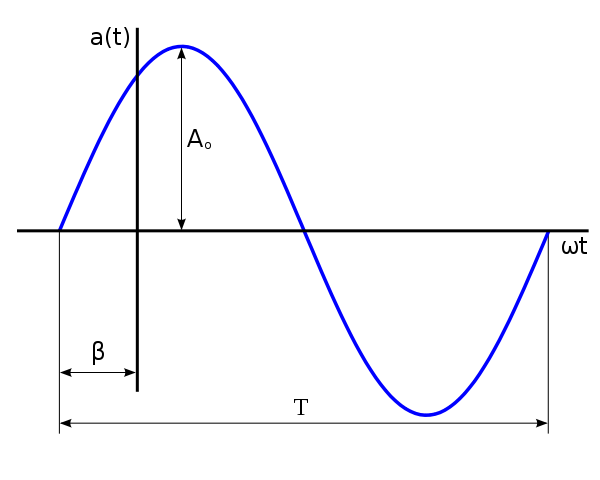
\includegraphics[scale=0.5]{Imagenes/600px-OndaSenoidal.png}
    \caption{Parámetros característicos de una oscilación sinusoidal.}
    \label{fig:ondaSenoidal}
\end{figure}

\section{Resistencia e Impedancia}

La impedancia (Z) es una medida de oposición que presenta un circuito a una corriente cuando se aplica una tensión. La impedancia extiende el concepto de resistencia a los circuitos de corriente alterna (CA), y posee tanto magnitud como fase, a diferencia de la resistencia, que sólo tiene magnitud.\\

%\section{Circuito a resolver}

%\begin{figure}[h!]
 %   \centering
   % \includegraphics{}
  %  \begin{circuitikz}
%\draw

%(-1,0)--(-1,-1)
%(-1,-1) to[V,l=$28v$](-1,-2) 
% (-1,-2)--(-1,-3)
 
% (-1,-3)--(2,-3)
 
% (-1,0) to[R,l=$50 \Omega $](2,0)
 
 
 %(2,-3)to[R,l=$5 \Omega$](2,0)
 
 %(2,0)--(4,0)
 %(2,-3)--(4,-3)
 
  %(4,-3)to[R,l=$10 \Omega$](4,0)
 
 
%;

%\draw[thick,arrows=->]
%(2.5,0)--(2.5,-1)
%;
 
%\end{circuitikz}
 %   \caption{Circuito a resolver}
  %  \label{fig:circuito}
%\end{figure}

%\subsection{Resultados}

%Para resolver el circuito se hicieron equivalente los resistores de 5 y 10 $\Omegas$ para obtener el voltaje en esas ramas, así se pudo deducir la corriente en la rama del resistor de 50 $\Omega$ y el circuito equivalente, posterirmente se usaron las leyes de Kirchhoff para deducir los voltajes y las corrientes respectivamente.

%\begin{table}[h!]
%\centering

%\begin{tabular}{|c|c|c|}
%\hline
%Componente & V {[}V{]} & I {[}A{]} \\ \hline
%R 50       & 26.25     & 0.525     \\ \hline
%R 10       & 1.75      & 0.173     \\ \hline
%R 5        & 1.75      & 0.352     \\ \hline
%V fuente   & 28        & 0.525     \\ \hline
%\end{tabular}
%\caption{Tabla de Resultados}
%\label{tabla-resultados}

%\end{table}


\bibliographystyle{plain}
\bibliography{Previo1.bib}


\end{document}